% Inhaltsverzeichnis, Tabellen, Figuren und automatische Sprache

\chapter{ITFS}

%%%%%%%%%%%%%%%%%%%%%%%%%%%%%%%%%%%%%%%%%%%%%%%%%%%%%%%%%%%%%%%%%%%%%%%%%%%%%%%
%%%%%%%%%%%%%%%%%%%%%%%%%%%%%%%%%%%%%%%%%%%%%%%%%%%%%%%%%%%%%%%%%%%%%%%%%%%%%%%

\section{Inhalt}
\label{inh}

Den Inhaltsverzeichnis erstellt man mit dem Befehl \verb=\tableofcontents=. Dieser Befehl schreibt man vor den Kapiteln in der Hauptdatei.

%%%%%%%%%%%%%%%%%%%%%%%%%%%%%%%%%%%%%%%%%%%%%%%%%%%%%%%%%%%%%%%%%%%%%%%%%%%%%%%
%%%%%%%%%%%%%%%%%%%%%%%%%%%%%%%%%%%%%%%%%%%%%%%%%%%%%%%%%%%%%%%%%%%%%%%%%%%%%%%

\section{Automatische Referenzen}
\label{ar}

Ein sehr mächtiges Paket in Latex ist das Paket \verb=hyperref=. Mithilfe von diesem Paket kann man im erzeugten PDF Hyperlinks erstellen, auf welche man klicken kann und man wird dann direkt auf die referenzierte Stelle weitergeleitet. Zur Demonstration tue ich ein paar Labels verteilen und hier auf diese wie folgt referenzieren: \autoref{ar}, \autoref{inh}, \autoref{mk}, \autoref{mk_bla} und \eqref{mk_bla}. Man kann also Labels überall in den verschiedenen Dateien schreiben und solange alle Dateien über den Master verlinkt sind, kann man auf diese über den Befehl \verb=\autoref= auf alle Labels zugreifen und auf die jeweilige Objekte referenzieren mit automatischer Erkennung, was für Objekte diese sind (Kapiteln, Sektionen, Gleichungen, Bilder, Tabellen).

Nach meinem persönlichen Geschmack sehen die Farbkasten Scheiße aus. Alternativ kann man für das Paket hyperref die Option \verb=colorlinks= verwenden, um die Referenzen farblich zu markieren. 

Ich finde das wesentlich angenehmer, doch es geht etwas schöner. Man kann auch die Farben der Links nach ihrem Typ einstellen. 

%%%%%%%%%%%%%%%%%%%%%%%%%%%%%%%%%%%%%%%%%%%%%%%%%%%%%%%%%%%%%%%%%%%%%%%%%%%%%%%
%%%%%%%%%%%%%%%%%%%%%%%%%%%%%%%%%%%%%%%%%%%%%%%%%%%%%%%%%%%%%%%%%%%%%%%%%%%%%%%

\section{Tabellen}

Oft wird man irgendwelche Daten in schönen Tabellen angeben müssen wie z.B.

\begin{table}[!h]
	\centering
	\begin{tabular}{l|lc}
	\hline \hline
	Kategorien & Daten 1 & Daten 2 \\ \hline
	Kategorie 1 & 34567 & 3 \\
	Kategorie 2 & df & jkl 3453456 \\ \hline \hline
	\end{tabular}
	\caption{Tabelle mit irgendwelchen Daten}
	\label{itfs_tab_blabla}
\end{table}

die Ansammlung an Daten gegeben in \autoref{itfs_tab_blabla}. 

Manchmal wird man auch Sachen aufzählen wollen aber nicht in solchen Datentabellen angeben, sondern bspw. Stichpunkte aufzählen. Dies kann man mit der Umgebung \verb=enumerate= machen, bspw.
\begin{enumerate}[~~~a)]\itemsep=-2mm
	\item die Rosen sind rot
	\item der Himmel ist blau
	\item die Bananen sind gelb, die Tomaten sind auch rot, ich habe gerade Hunger Hunger Hunger, habe Hunger Hunger Hunger, habe Hunger Hunger Hunger, habe Durst!
\end{enumerate}
Diese Umgebungen können gut mithilfe des Paketes \verb=enumitem= eingestellt werden. Nützlich ist auch die \verb=itemize=-Umgebung
\begin{itemize}\itemsep=-1mm
	\item die Rosen sind rot
	\item der Himmel ist blau
	\item die Bananen sind gelb, die Tomaten sind auch rot, ich habe gerade Hunger Hunger Hunger, habe Hunger Hunger Hunger, habe Hunger Hunger Hunger, habe Durst!
\end{itemize}
Wieder zurück zu den Datentabellen. Manchmal wird man etwas Pech haben und eine Tabelle mit suuuuuuuper vielen Daten angeben müssen, die aber leider nicht auf eine Seite passen wird. Für solche Fällen empfiehlt es sich die \verb=longtabel=-Umgebung zu verwenden, wie in \autoref{lt}.

\begin{center}
\begin{longtable}{l|l|l}

% \baselinestretch{1.5}

 \hline \hline
 $i^3$ & $2i^3$ & $3i^3$ \bigstrut \\ \hline
 \endfirsthead
 
 \multicolumn{3}{c}{\tablename\ \thetable{} -- fortgesetzt von voriger Seite} \\
 \hline
 $i^3$ & $2i^3$ & $3i^3$ \bigstrut \\ \hline 
 \endhead
 
 \hline
 \multicolumn{3}{c}{Wird auf nächste Seite fortgesetzt} \\ \hline
 \endfoot
 
 \hline \hline
 \caption{Long Table}
 \label{lt}
 \endlastfoot
 
 1 & 2 & 3 \\
 8 & 16 & 24 \\
 27 & 54 & 81 \\
 64 & 128 & 192 \\
 125 & 250 & 375 \\
 216 & 432 & 648 \\
 343 & 686 & 1029 \\
 512 & 1024 & 1536 \\
 729 & 1458 & 2187 \\
 1000 & 2000 & 3000 \\
 1331 & 2662 & 3993 \\
 1728 & 3456 & 5184 \\
 2197 & 4394 & 6591 \\
 2744 & 5488 & 8232 \\
 3375 & 6750 & 10125 \\
 4096 & 8192 & 12288 \\
 4913 & 9826 & 14739 \\
 5832 & 11664 & 17496 \\
 6859 & 13718 & 20577 \\
 8000 & 16000 & 24000 \\
 9261 & 18522 & 27783 \\
 10648 & 21296 & 31944 \\
 12167 & 24334 & 36501 \\
 13824 & 27648 & 41472 \\
 15625 & 31250 & 46875 \\
 17576 & 35152 & 52728 \\
 19683 & 39366 & 59049 \\
 21952 & 43904 & 65856 \\
 24389 & 48778 & 73167 \\
 27000 & 54000 & 81000 \\
 29791 & 59582 & 89373 \\
 32768 & 65536 & 98304 \\
 35937 & 71874 & 107811 \\
 39304 & 78608 & 117912 \\
 42875 & 85750 & 128625 \\
 46656 & 93312 & 139968 \\
 50653 & 101306 & 151959 \\
 54872 & 109744 & 164616 \\
 59319 & 118638 & 177957 \\
 64000 & 128000 & 192000 \\
 68921 & 137842 & 206763 \\
 74088 & 148176 & 222264 \\
 79507 & 159014 & 238521 \\
 85184 & 170368 & 255552 \\
 91125 & 182250 & 273375 \\
 97336 & 194672 & 292008 \\
 103823 & 207646 & 311469 \\
 110592 & 221184 & 331776 \\
 117649 & 235298 & 352947 \\
 125000 & 250000 & 375000 \\
\end{longtable}
\end{center}

%%%%%%%%%%%%%%%%%%%%%%%%%%%%%%%%%%%%%%%%%%%%%%%%%%%%%%%%%%%%%%%%%%%%%%%%%%%%%%%
%%%%%%%%%%%%%%%%%%%%%%%%%%%%%%%%%%%%%%%%%%%%%%%%%%%%%%%%%%%%%%%%%%%%%%%%%%%%%%%

\section{Figuren}

In jedem Dokument wird man vieles bildlich darstellen, motivieren oder erklären wollen, sodass das Hinzufügen von Bildern unvermeidlich ist. Hierzu bietet sich die \verb=figure=-Umgebung in Kombination mit *.eps-Figuren an, wie in \autoref{itfs_fig_plot}.

\begin{figure}[!ht]
	\centering
	a) 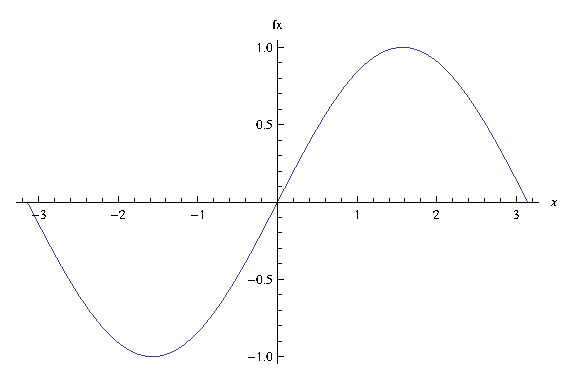
\includegraphics[width=0.4\textwidth]{pics/plot.eps} \quad
	\psfrag{x}{$x$}
	\psfrag{fx}{$f(x)=\sin(x)$}
	b) 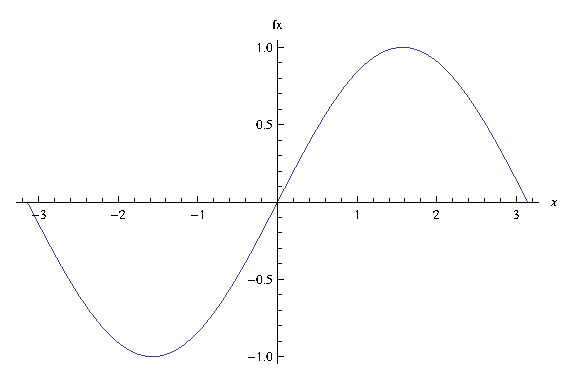
\includegraphics[width=0.4\textwidth]{pics/plot.eps}
	\caption{Irgendein EPS-Bild in a) und in b) mit Verwendung von psfrag}
	\label{itfs_fig_plot}
\end{figure}

%%%%%%%%%%%%%%%%%%%%%%%%%%%%%%%%%%%%%%%%%%%%%%%%%%%%%%%%%%%%%%%%%%%%%%%%%%%%%%%
%%%%%%%%%%%%%%%%%%%%%%%%%%%%%%%%%%%%%%%%%%%%%%%%%%%%%%%%%%%%%%%%%%%%%%%%%%%%%%%

\section{Automatische Sprache}

Bis jetzt heißen all unsere schönen Referenzen \autoref{mk}, \autoref{itfs_fig_plot} und das Inhaltsverzeichnis ist auch auf Englisch. Das alles kann man auf Deutsch umstellen mit dem Paket \verb=ngerman=. Hiermit ist das Inhaltsverzeichnis auf deutsch, die chapters werden zu Kapiteln und alle captions sind ebenfalls auf deutsch. Aber die Referenzen immer noch auf Englisch. Um dies zu ändern, muss zum Paket \verb=hyperref= die Option \verb=ngerman= dazu gegeben werden, dann stimmt alles.

%%%%%%%%%%%%%%%%%%%%%%%%%%%%%%%%%%%%%%%%%%%%%%%%%%%%%%%%%%%%%%%%%%%%%%%%%%%%%%%
%%%%%%%%%%%%%%%%%%%%%%%%%%%%%%%%%%%%%%%%%%%%%%%%%%%%%%%%%%%%%%%%%%%%%%%%%%%%%%%

\section{Listen der Tabellen und Figuren}

Alle Tabellen und Figuren können am Ende der Arbeit in automatisch generierten Listen angegeben werden.